\documentclass[
	11pt
] {article}

\usepackage[
	a4paper,
	left=1.5cm,
	right=1.5cm,
	top=2.5cm,
	bottom=2.5cm,
	headheight=1cm
] {geometry} %for setting margin

\usepackage{fancyhdr} %for header and footers
\usepackage{parskip} %for leaving some space after paragraphs


% Math
\usepackage{mathtools} %helps to number equations
\usepackage{siunitx} % Units of measurement


% For graphs and advanced diagrams
\usepackage{tikz} %the drawing library
\usetikzlibrary{positioning} %some auxilary to the drawing library
\usetikzlibrary{math} %helps to define variables in the tikz

\usepackage{authblk} %authors and their affiliations

% Basic graphics
\usepackage{float} %to force the figure to be in a place among the text
\usepackage{graphicx} %for include graphics
\usepackage{caption} %better referencing to labels
\usepackage{subcaption}  %helps with multiple pictures in a figure


% Language and Font package: COMMENT THESE FOR ENGLISH ONLY
\usepackage[T2A]{fontenc} %[RUS] loads cyrillic characters
\usepackage[russian]{babel} %[RUS] changes date heading 'abstract' to Russian
\usepackage[utf8]{inputenc} %[RUS] to force utf-8 encoding
\usepackage{hyperref}


%-----------------------------------------------------------------------

\renewcommand\thesubfigure{\asbuk{subfigure}} %[RUS] for renaming subfigures to russian
\sisetup{output-decimal-marker = {,}} %[RUS] changes all ordinary decimal separator to rassiky commas
\pagestyle{fancy}
\graphicspath{{figures/}}


\newcommand\titleshort{Most popular commentator}

\author[1]{Jamclub}

\affil[1]{Физтех-confessions}

\title{Физтех-сonfessions, the most popular commentator of 2024}
\fancyhead{}
\fancyhead[L]{Физтех-сonfessions}
\fancyhead[C]{\titleshort}
\fancyhead[R]{\the\year}



\begin{document}

\maketitle
\renewcommand{\arraystretch}{1.3}

\begin{abstract}
	Based on the number of likes each comment received, this report determines who is the most popular commentator of физтех-confessions. Comparison between the influence of the the top few commentators and the rest of the community is also made.
\end{abstract}

\tableofcontents


\section{Introduction and Motivation}
	2024 was a great year! Физтех-confessions was used:
	\begin{enumerate}
		\item To confess love and sins
		\item As a means to procrastinate from doing work
		\item To pass depression
		\item To get daily dose of cringe because the brain demands it, just as our body demands \num{2.5}L of water everyday
		\item To share some brilliant memes.
	\end{enumerate}
	We can obviously discuss the most liked posts, which will be a discussion on the created objects, but here I am more interested on the people, who keeps the community alive, so who is the most popular commentator of 2024?

\section{Collection of Data}
	\subsection{Basic statistics on the source}
		\begin{enumerate}
			\item Time period = 08.05.2023 - 11.12.2024.
			\item Number of posts analyzed = 5000.
			\item Number of comments analyzed = 17753.
			\item Number of authors of comments = 1778
		\end{enumerate}

		An amateur code \cite{code-scrape-py} was used to iterate through all posts backwards in time, starting from 11.12.2024 until 5000 posts were successfully read, and the number of likes on each comment and the author of the comment was recorded and put onto our main table. Instead of 2024, 1.5 year worth of data was used, because the физтех-confessions had change of admins and other breaks this year, and more data is always good for statistics.


	\subsection{Sources of errors}
		A python code was used to browse vk and collect data instead of vk.api. The code could not read some of the comments if the page of the post had a lot of comments. Because such comments are collapsed and the code was not smart enough to click on buttons and expand to read all comments. Since the sample size is still very large, such errors do not distort the conclusions. Vk.api would give correct data but it was not used due to task being too technically difficult in nature given the aim is to only guess the most popular commentator.



		h-index: the total number  of comments - h, such that the number of likes in each of these comments is greater than or equal to h.

		popularity = normalized\_count\_likes * normalized\_count\_comments * h-index


\section{Results and Discussion}
\subsection{The most Liked commentator (count\_likes)}
	Definitions:
	\begin{itemize}
		\item count\_likes: the total number of likes an author received for the whole data.
		\item serial: the rank when the table is sorted based on count\_likes.
		\item author: the commentator, or the author of a comment.
	\end{itemize}

	\begin{table}[H]
		\centering
		\caption{Top-20 authors with most likes \cite{sheet-count-likes}.}
		\label{table-count-likes}
		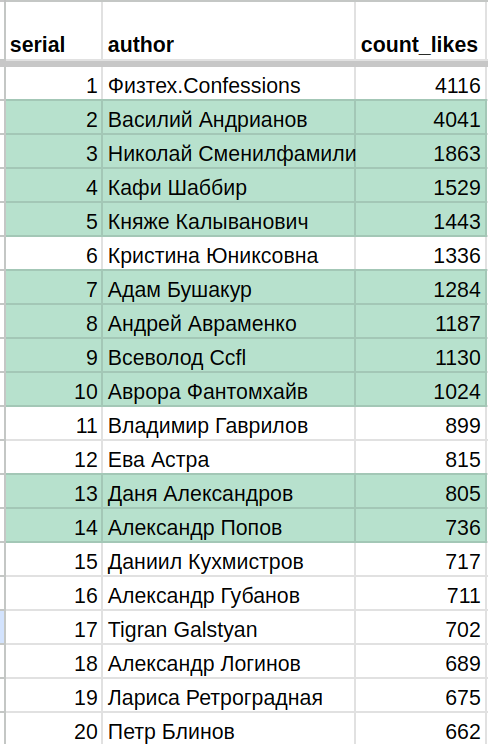
\includegraphics[width=0.4\textwidth]{table-count-likes-488}
	\end{table}

	\begin{table}[H]
		\centering
		\caption{Basic statistics on number of likes, comments and authors.}
		\label{table:basic-stats-number-likes-comments-author}
		\begin{tabular}{| p{5cm}  c |} % or ccS
			\hline
			Total number of likes & \num{75881} \\
			Total number of comments & \num{17753} \\
			Total number of authors & \num{1778} \\
			\hline
			Average number of likes per comment & \num{4.27} \\
			Average number of comments per author & \num{9.98} \\
			\hline
			\hline
			Number of likes received by the top-10 authors, (green rows in Table \ref{table-count-likes}) & \num{15042} \\
			Number of comments written by the top-10 authors & \num{2291} \\
			Average number of likes per comment for top-10 author & \num{6.57} \\
			\hline
			Percent of comments written by top-10 authors & \num{12.9}\% \\
			Percent of likes by top-10 & \textbf{\num{19.8}}\% \\
			\hline
			\hline
			Number of likes received by the top-40 authors & \num{35536} \\
			Number of comments written by the top-40 authors & \num{7846} \\
			Average number of likes per comment for top-40 author & \num{4.5} \\
			\hline
			Percent of comments written by top-40 authors & \num{44.2}\% \\
			Percent of likes by top-40 & \textbf{\num{46.8}}\% \\
			\hline
		\end{tabular}
	\end{table}

	\begin{figure}[H]
		\centering
		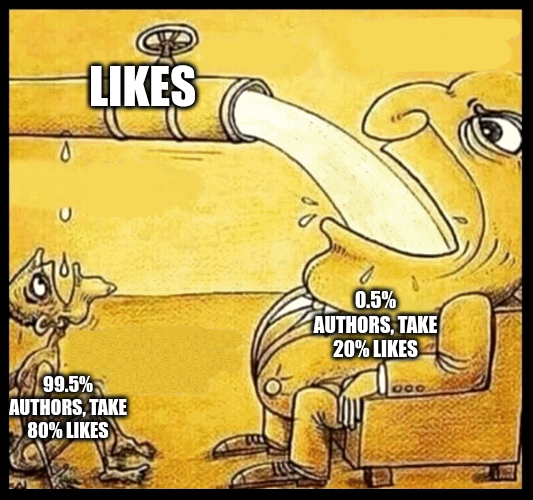
\includegraphics[width=0.5\textwidth]{fig-small-author-take-almost-all-likes}
		\caption{A few authors take a lot of likes}
		\label{fig-small-author-take-almost-all-likes}
	\end{figure}

	We can also say that half of the comment activity comes from just 40 authors. Now for simplicity, let us consider only the top-500 authors, and will have a look at the distribution curve on how the likes are distributed amount these 500 authors. It is reasonable to take the top-500 instead of all \num{1778} because, the 500th author when sorted on count\_likes had only 18 likes in total. We can assume that 501st author and on wards do not have much desire to get likes, therefore it will not be fair to add them to the distribution curve and conclude that the like distribution among the rich and poor is very large. By rich, of course we mean, those who took a large share of the total likes, and by poor who took a small share of the total likes. Also, the top-500 contribute to \num{93}\% of the total likes, so completely removing the others does not leave a big proportion of the data out.

	\begin{figure}[H]
		\centering
		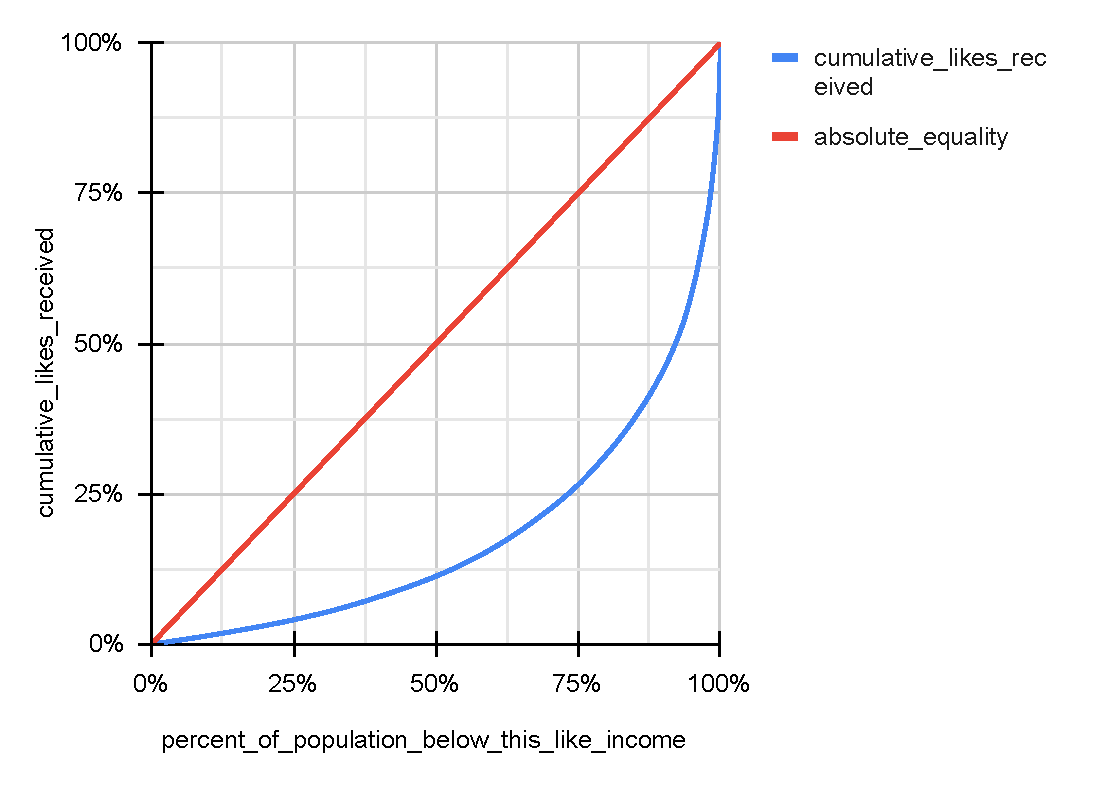
\includegraphics[width=0.8\textwidth]{fig-gini-calculation}
		\caption{Determination of gini-coefficient \cite{wikipedia-gini}}
		\label{fig-gini-calculation}
	\end{figure}

	We have used 500 authors to form the gini-distribution, so the top 10 are the top \num{2}\% wealthy men and the top 40 are the top \num{8}\% wealthy men in физтех-confessions. We see that their like contribution is \num{26.7}\% and \num{50.1}\% respectively. This is considering the top-500 authors, when we compare this with table \ref{table:basic-stats-number-likes-comments-author}, which includes all the \num{1778} authors, the percent of contribution of likes is not very different \cite{sheet-calc-gini-coefficient}.

	We determine our inequality by the gini-coefficient \cite{wikipedia-gini}, which is calculated from figure \ref{fig-gini-calculation}, here the gini coefficient is \num{0.64} which makes it similar to South Africa, which has the highest income inequality in the world. In other words in South Afria, the top \num{2}\% richest men take \num{26.7}\% of the country's annual wealth, and the top \num{8}\% of the the richest men takes \num{50.1}\% of the country's annual wealth, just as it is the case with физтех-confessions, except luckily it is not food, water and iron, but just the amount of adrenaline rush from receiving notifications of a comment being liked. For comparison, we can look at other countries:
	\begin{table}[H]
		\centering
		\caption{Gini-coefficients of various countries}
		\label{table:gini-countries}
		\begin{tabular}{| c | c | c |} % or ccS
			\hline
			rank & country & gini-coefficient \\
			\hline
			1 & Физтех-confessions & \num{0.64} \\
			2 & South Africa & \num{0.63} \\
			3 & USA & \num{0.39} \\
			4 & Russia & \num{0.36} \\
			5 & Sweden & \num{0.29} \\
			6 & Norway & \num{0.23} \\
			\hline
		\end{tabular}
	\end{table}

	However note that we talk about South Africa based on our curve of физтех-confessions since we have almost the same gini-coefficient, but the exact distribution for the top \num{2}\% and the top \num{8}\% can be slightly different because gini-coefficient is due to the area between the red and the blue curve, this coefficient can be same due to the same area but actual blue curves can be slightly different.

\subsection{The most Depressed commentator (count\_comments)}
	Definitions:
	\begin{itemize}
		\item rank: position based on a characteristic for a local table, while the serial is always the rank when the table was sorted according to count\_likes.
		\item count\_comments: the total number of comments an author wrote.
		\item sr-difference = serial - rank is the difference between the the positions in the table of count\_likes and int this table. We would want to know if we change the measure based on which we sort the table how much does it differ from the table which was sorted based on the number of likes.
	\end{itemize}

	\begin{table}[H]
		\centering
		\caption{Top-20 authors with most comments, \cite{sheet-count-comments}.}
		\label{table-count-comments}
		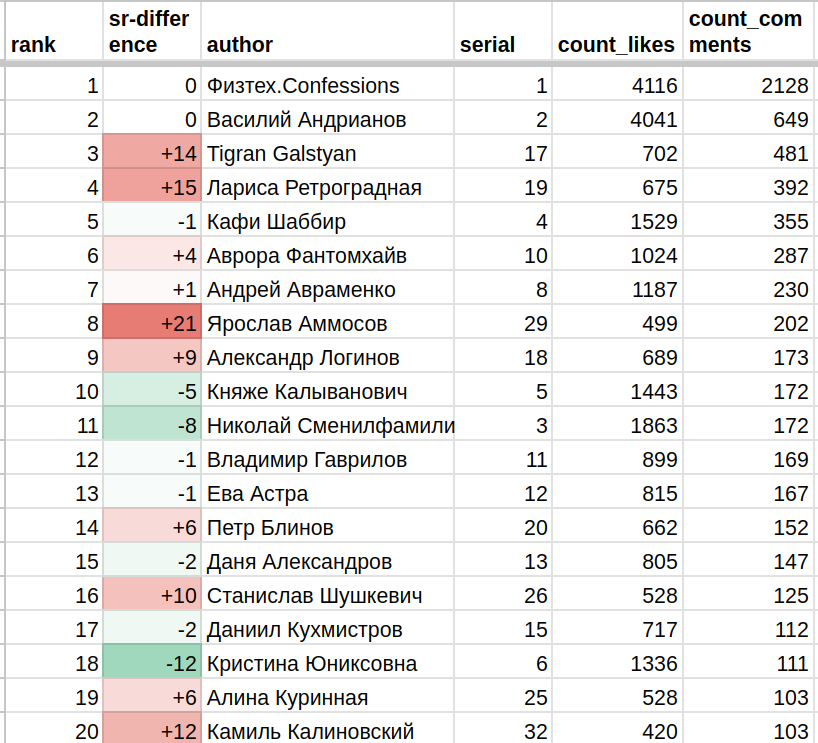
\includegraphics[width=0.7\textwidth]{table-count-comments-818}
	\end{table}

	Certainly the most depressed student in физтех writes the most amount of comments. And now by the legendary sr-difference we see that Tigran Galstyan has moved up 14 places as compared to Table \ref{table-count-likes}. Лариса Ретроградная has also moved up a massive amount of 15 places it is because her comments are self contradictory, trolling or just toxic. Ярослав Аммосов has moved up many places it is because his comments are usually emojis or compliments appreciating the post or a comment of another author. Кафи Шаббир has moved down one place which indicates that his ratio of quality over quantity if not neural slightly good for the community. Николай Сменилфамилиюнавзрослуюсерьёзную has gone down by 8 places which means his quality over quantity is pretty high.

	\begin{figure}[H]
		\centering
		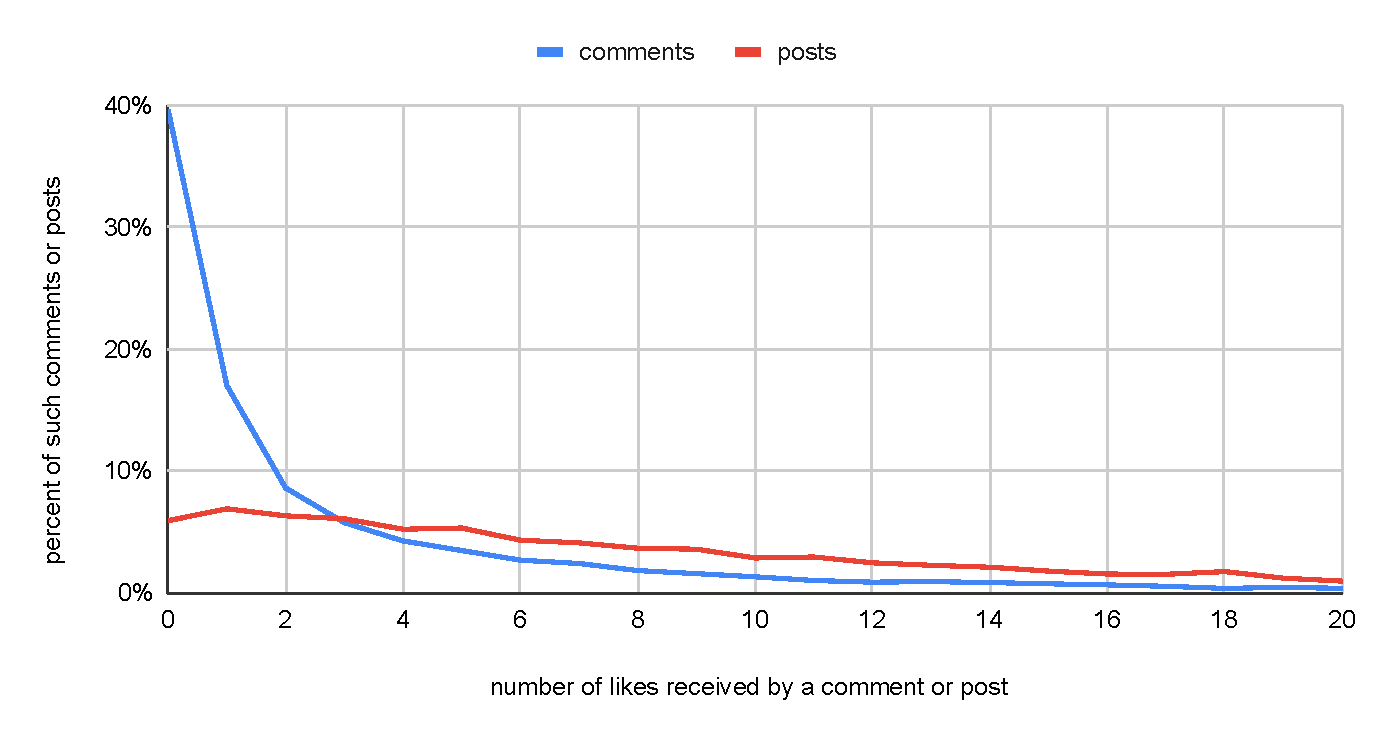
\includegraphics[width=1\textwidth]{fig-proportion-of-posts-or-comments-with-certain-likes}
		\caption{Percent of comments or posts which has the given number of likes.}
		\label{fig-proportion-of-posts-or-comments-with-certain-likes}
	\end{figure}
	Now let us see how the likes on comments are distributed. In other words what percent of comments have 0 likes and what percent of comment have more than 5 likes. In figure \ref{fig-proportion-of-posts-or-comments-with-certain-likes}, if you read for the blue curve $(x, y) = (2, 10\%)$, it means that \num{10}\% of the comments have \num{2} likes. The red curve is the like distribution for the posts on confessions. As expected the curve for the posts decreases smoothly and maintains a large enough positive value for $\num{20} + $ likes, but for comments $\num{40}\%$ of the comments have 0 likes and the proportion of comments as the number of likes increases falls much more rapidly than that of физтех-confessions posts.

	\begin{figure}[H]
		\centering
		\begin{subfigure}[b]{0.49\textwidth}
			\centering
			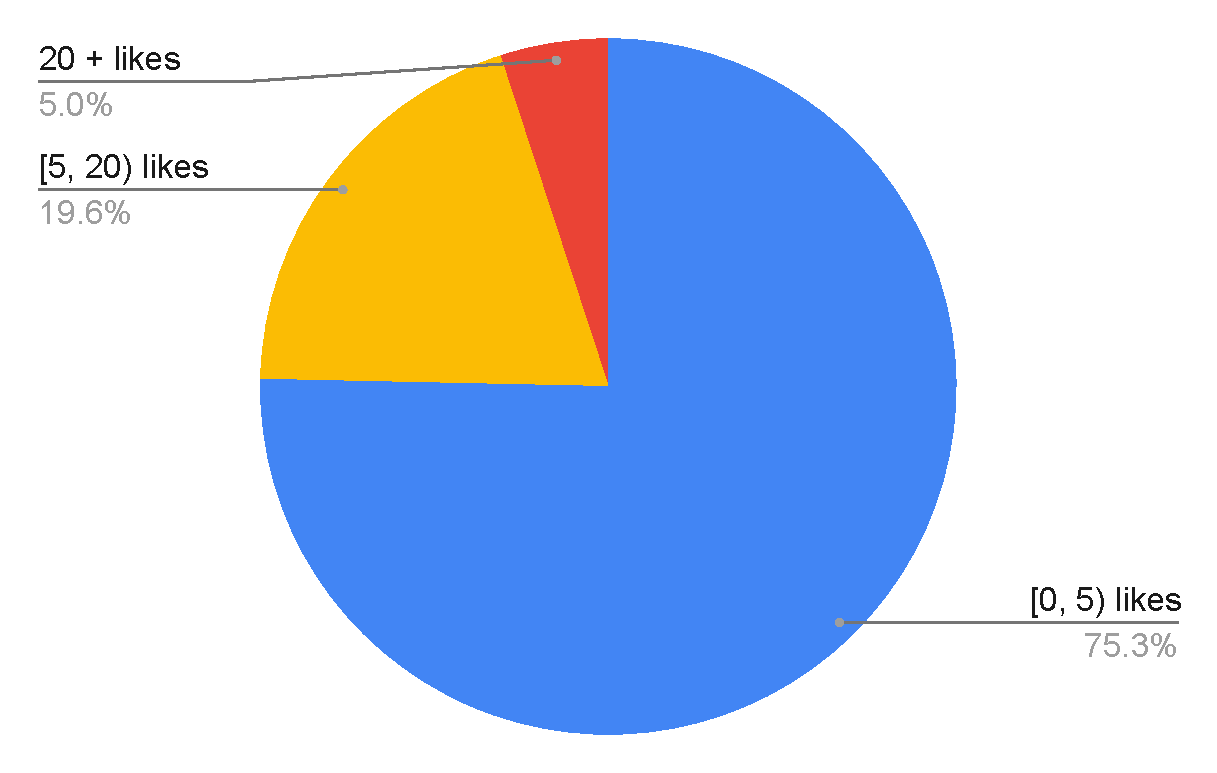
\includegraphics[width=\textwidth]{fig-proportion-of-comments-by-likes}
			\caption{Comments}
		\end{subfigure}
		\hfill
		\begin{subfigure}[b]{0.49\textwidth}
			\centering
			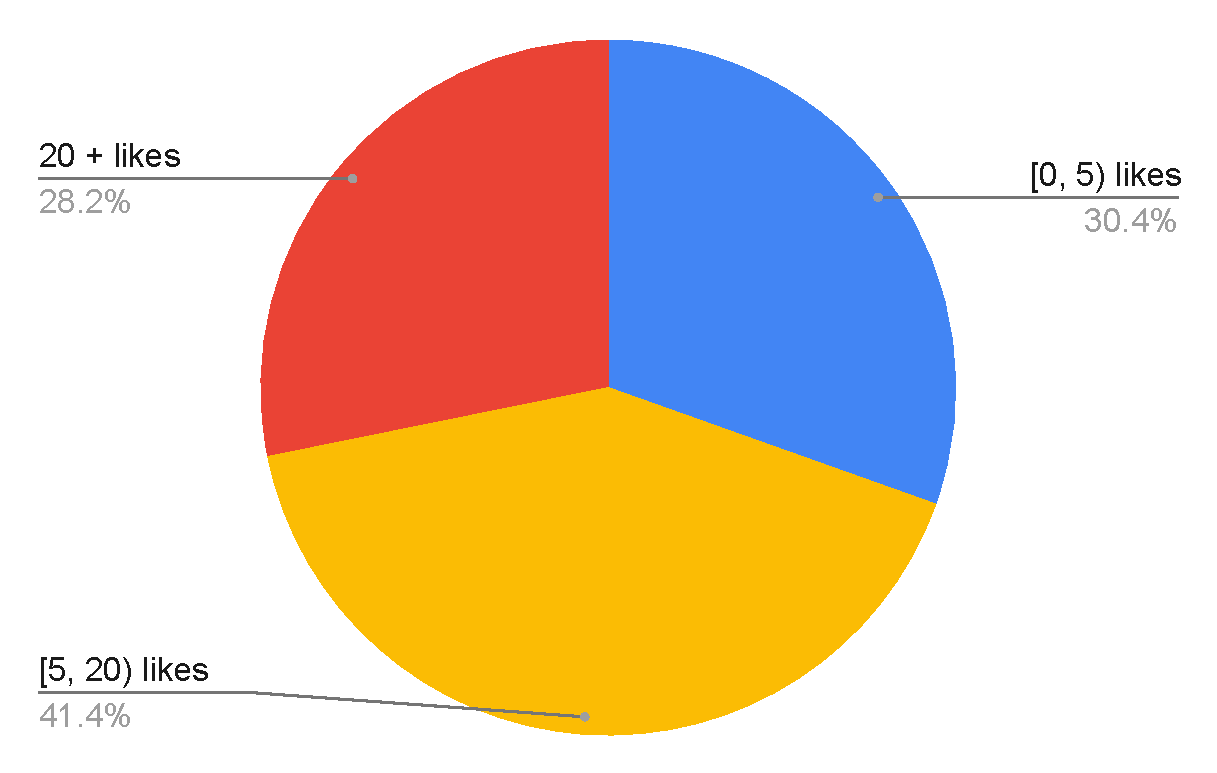
\includegraphics[width=\textwidth]{fig-proportion-of-posts-by-likes}
			\caption{Posts}
		\end{subfigure}
		\caption{Proportion of likes for comments and posts.}
		\label{fig-proportion-of-comments-or-posts-by-likes}
	\end{figure}

	In figure \ref{fig-proportion-of-comments-or-posts-by-likes}, we see that only \num{5}\% of the comments have more than \num{20} likes while, \num{28.2}\% of the posts have more than \num{20} likes.

\subsection{The most Sigma commentator (density)}
	Definitions:
	\begin{itemize}
		\item density = count\_likes / count\_comments, is the number of likes per comment written by the author.
	\end{itemize}

	\begin{table}[H]
		\centering
		\caption{Top-40 authors sorted according to density \cite{sheet-density}}
		\label{table-density}
		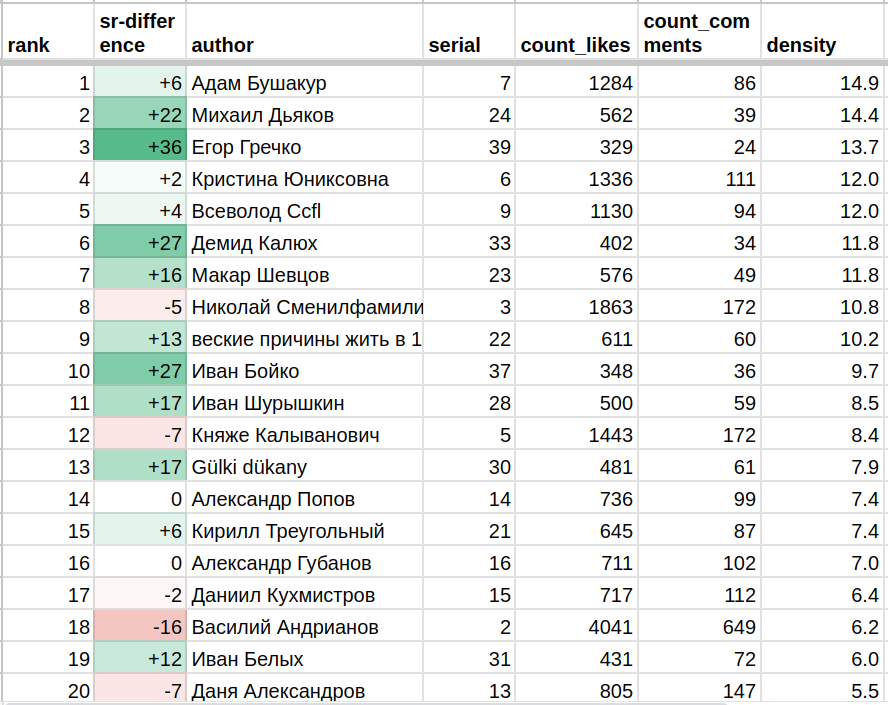
\includegraphics[width=0.75\textwidth]{table-density}
	\end{table}

	This The number of likes and the number of comments certainly does not give us all the information. These are sigma's who keep silent, but when they speak something, it caries a lot of value. Кафи Шаббир completely flew away form the list ending up at 30th place. Адам Бушакур is certainly the sigma here, his density given the amount of comments he wrote can be matched by a few.

	\begin{figure}[H]
		\centering
		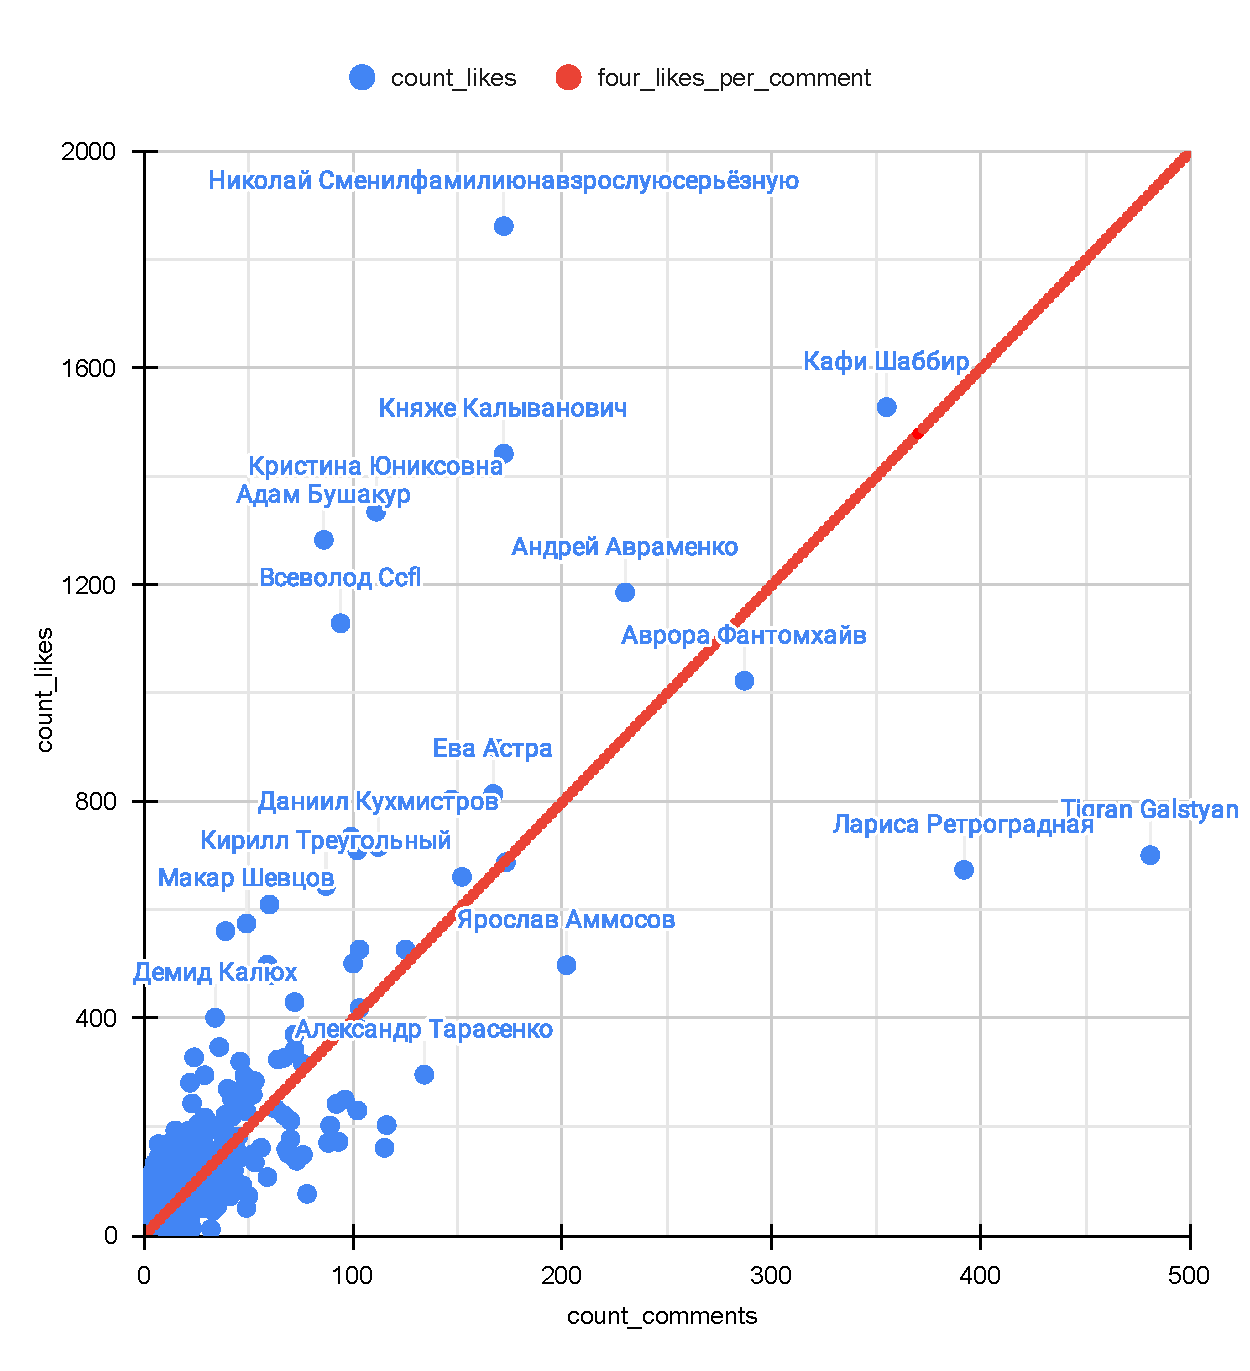
\includegraphics[width=0.7\textwidth]{fig-count-likes-comments-author-points}
		\caption{Number of likes vs comments points for different authors.}
		\label{fig-count-likes-comments-author-points}
	\end{figure}


	In figure \ref{fig-count-likes-comments-author-points} we can draw a line called the line of four\_likes\_per\_comment, this line represents the average density of all comments of all authors. Here Физтех.Confessions and Василий Андрианов were excluded to keep the scales of axes reasonable. Кафи Шаббир just managed to keep himself above this line while Аврора Фантомхайв is close to this line but below it. Now based on this line we can place our beloved authors into 4 zones.

	\begin{figure}[H]
		\centering
		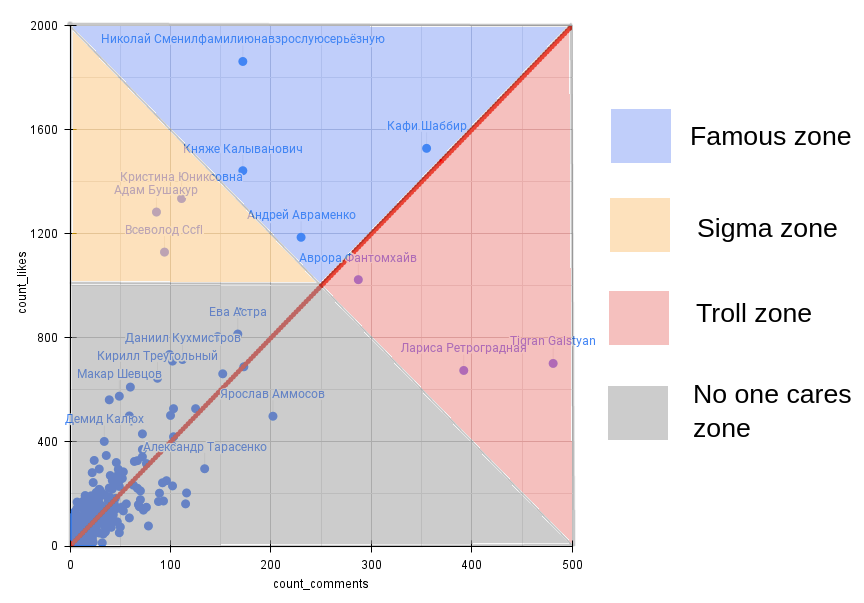
\includegraphics[width=0.9\textwidth]{fig-likes-vs-comments-divided-into-zones}
		\caption{The four zones on likes vs comments plot of various authors.}
		\label{fig-likes-vs-comments-divided-into-zones}
	\end{figure}

	\begin{enumerate}
		\item \textbf{Famous zone}: authors of this zone are famous.
		\item \textbf{Sigma zone}: authors of this zone many not be known to all but those who know them respect these authors' comments a lot.
		\item \textbf{Troll zone}: authors in this zone write a lot of troll comments.
		\item \textbf{No one cares zone}: not a lot of audience cares or knows about the authors in this zone.
	\end{enumerate}

	\subsection{The most cringe commentator (reverse density)}


	We can possibly divide the count like and count comment graph into 4 zones.

\subsection{The best Female commentator}
\subsection{The most Productive Commentator}

	H-index depends on the number of likes and the comment density
\section{Conclusion}
	This report was prepared without the consent to publish name or profile pictures of the commentators. If you have a problem with it, you can cry about it.

\bibliographystyle{plain.bst}
\bibliography{reference}
\end{document}
